\chapter{Introduction} \label{ch:intro}

%% =====================================================================================
%%
%%              G E N E R A L  I N T R O D U C T I O N
%%
%% =====================================================================================

%% From Just
A pair of massive stars at the end of their evolution undergo \acp{SN} explosions, and 
if stars are sufficiently massive, a pair of compact objects orbiting each other is formed. 
One of the possible outcomes, is a pair of \acp{NS}, compact, but heavy objects sustained 
against gravitational collapse by the neutron degeneracy pressure. 
The theory of \ac{GR} predicts that the orbit of the system shrinks, as \acp{NS} loose energy 
and angular momentum to \acp{GW}. The stars inspiral until they collide at the last orbit. 
%ejecting a small fraction of matter into the Universe, leaving a \pmerg{} remnant.


The high compactness of \acp{NS} leads to an energetic, explosive merger, where a small 
fraction of the \ac{NS} matter is ejected from the system at mildly relativistic 
velocities. 
Additionally, the massive \pmerg{} remnant and sorrounding it gravitationally bound 
matter are subjected to complex dynamical interactions, weak processes and magnetically induced 
turbulence, that might induce additional matter outflows. This makes the \ac{BNS} mergers 
strong contributors to the cosmic chemical evolution. 
The matter ejected at/after mergers, \ie, ejecta, has unique properties, rarely found in other 
astrophysical sites. Specifically, the abundance of free neutrons allow for the so-called 
rapid neutron capture process (\rproc{}), 
The \rproc{}, that is responsible for the production of the heaviest elements in the 
Universe, lanthanides and actinides. 

%Mergers of \acp{BNS} are at the center of a variety of physical processes in astrophysics.
Wide range of possible types and properties of ejecta lead to a similarly broad 
range in \ac{EM} counterparts to \ac{BNS} mergers. For instance, the heavy elements 
produced via \rproc{} \nuc{} eventually decay, powering the quasi-thermal \ac{EM} 
counterpart, \ac{kN}. Additionally, it \ac{BNS} mergers are expected to produce 
powerful jets, that can be observed as \acp{SGRB}. Moreover, expanding into \ac{ISM} 
medium, \ac{BNS} merger ejecta is expected to generate non-thermal, long-lasting 
afterglow emission. 
%Perhaps, two of the most 
%well studied ones are the \ac{kN}, a thermal counterpart powered by the decay of 
%newly synthesized heavy elements in the ejecta, and \acp{SGRB}, generally non-thermal 
%emission from the ultrarelativistic collimated outflow, formed after the merger. 
Together with \ac{GW} emission, these signals allow to study the processes occuring 
at mergers to a great detains, origin of the \ac{SGRB}, cosmic chemical evolution, 
and, perhaps most importantly, they provide unique constraints on the theory of gravity 
and density of matter at many times the nuclear saturation densities. 
%Study of these \ac{EM} counterparts in conjuncture with \acp{GW} emission allows to 
%gain unique insigts into the inner workings of the \ac{BNS} merger and previously 
%unobtainable constraints on the theory of gravity, the properties of matter at 
%supranuclear densities, origin of the \ac{SGRB}, cosmic chemical evolution. 



In August 2017, the first \ac{BNS} merger was observed 
as a source of \ac{GW} waves by \ac{LIGO}/Virgo, \GW{}. The unprecedented \ac{EM} 
follow-up campaign, spanning hundreds of observatories across the world lead to 
the identification of the merger \ac{EM} counterparts: \ac{kN}, \AT{} and 
\ac{SGRB}, \GRB{} 
\citep{TheLIGOScientific:2017qsa,Abbott:2018wiz,GBM:2017lvd}. 
%
\acp{GW} shed light on the properties of cold matter 
at supernuclear densities, the \ac{NS} \ac{EOS} 
\citep{Hinderer:2009ca,Damour:2012yf,DelPozzo:2013ala}, while 
the properties of matter at densities several times that of the 
nuclear matter, as well as the astrophysical implications of the merger 
were largely derived from the \ac{EM} signals 
\cite{Alexander:2017aly,Villar:2017wcc,Hajela:2019mjy}. \red{add proper refs}


The complexity, non-linearity, non-stationarity and multidimensionality of physical 
processes operating at \ac{BNS} mergers on a wide range of scales of length and time 
implies that self-consistent, quantitative studies are only possible with numerical 
simulations 
\citep{Sekiguchi:2011zd,Wanajo:2014wha,Foucart:2015gaa,Palenzuela:2015dqa,Sekiguchi:2016bjd,Kiuchi:2017zzg,Radice:2017zta,Fujibayashi:2017puw,Radice:2018pdn}.
These simulations, performed with \ac{NR} codes that took years, sometimes 
decades to develop and test, are very computationally expensive, rare, and require detailed 
postprocessing and analysis. 
%
Moreover, the self-consistent modeling of the \ac{BNS} merger and its \ac{EM} counterparts 
is still beyond the reach of modern methods. Generally, the short-term (hundred of milliseconds) 
evolution of the merger itself is handled with \ac{NR} codes while the 
\nuc{} and \ac{EM} emission are computed after, in postprocessing. 
%Strengthening the connection between these methods is one of the goals of this thesis. 
%
%In the following sections we sketch the astrophysical background to clarify the 
%context of our study and we conclude the chapter by summarizing the main points of 
%motivation for this thesis and its structural arrangement.

In this thesis we postprocess a large set of \ac{NR} \ac{BNS} merger simulations, 
performed with the state-of-the-art \ac{NR} code, \wisky{}, and targeted to the 
\GW{} (with corresponding binary parameters).
%
We focus on the \pmerg{} matter dynamics and properties of ejecta. 
We asses the nucleosynthetic yields in the ejecta, placing them into astrophysical 
context. Using the \ac{kN} model, developed by \citet{Perego:2017wtu}, we analyze 
the \ac{EM} signatures of our \ac{BNS} merger models, comparing them with \AT{}. 
Additionally, we develop a new code to model non-thermal emission from ejecta 
expanding into \ac{ISM}, apply it to the outcome of the merger simulations and 
compare the results with recently observed change in \ac{SGRB} emission. 
%
The main goal of our study is to strengthen the link between the ab-inito 
numerical relativity simulations and observations of \ac{EM} signatures of mergers, 
and in doing so, provide better constraints on the properties of \GW{} 
and ultimately, on the properties of matter and supranuclear densities.



%Single \acp{NS} are very compact but massive objects, 
%%where compactness $C_{i} = GM_i/R_i^2c^2\propto0.15$ and 
%for description of which the effects of \ac{GR} cannot be neglected. 
%%
%A pair of \acp{NS} orbiting each other slowly loses its 
%angular momentum to \acp{GW}. 
%%The timescale for the radiation reaction, however, 
%%is much longer than the orbital period for most of the inspiral and the 
%%system evolution can be considered adiabatic. 
%%For instance, the inspiral can be considered as a sequence of circular orbits. 
%%However, during last orbits before merger, the finite size (tides) and \ac{HD}
%%effects starts to become important. 
%The inspiral ends at the onset of the Roche lobe overflow, when the binary 
%reaches the mass-shedding limit \citep{Bejger:2004zx}.
%
%%% <<< From Radice Review >>>
%Mergers of \acp{BNS} are at the center of a variety of physical processes 
%in astrophysics.
%The first ever detection of such event by \ac{LIGO}/Virgo, \GW{}, 
%followed up by detections across \ac{EM} spectrum 
%have significantly advanced our understanding 
%of gravity, physics of dense matter, origins of \acp{SGRB} and \rproc{} elements 
%\citep{TheLIGOScientific:2017qsa,Abbott:2018wiz,GBM:2017lvd}. 
%%
%Specifically, while \acp{GW} shed light on the properties of cold matter 
%at supernuclear densities, the \ac{NS} \ac{EOS} 
%\citep{Hinderer:2009ca,Damour:2012yf,DelPozzo:2013ala}, 
%the properties of matter at densities several times that of the 
%nuclear matter, as well as the astrophysical implications of the merger 
%were largely derived from the \ac{EM} signals. 
%
%%Emitted during the inspiral, \acp{GW} delivered a plethora of information about  
%%\ac{NS} \ac{EOS} at supernuclear densities 
%%\citep{Hinderer:2009ca,Damour:2012yf,DelPozzo:2013ala}. 
%%%
%%The properties of matter at densities several times that of the 
%%nuclear matter, however, were not well constrained, as the \pmerg{} \ac{GW} 
%%was not detected. Future observations of the high frequency \pmerg{} signal 
%%will shed more light on these properties 
%%\citep{Sekiguchi:2011mc,Radice:2017lry,Most:2018eaw,Bauswein:2018bma}, 
%%constraining one of the main quantities, the tidal deformability.
%
%The \ac{EM} signal originates from the matter ejected during or after 
%the merger by a variety of physical processes, the so-called, ejecta.
%%
%The conditions within ejecta, are such that the rapid neutron capture (\rproc{}) 
%\nuc{}, responsible for the production of the heaviest elements in the Universe
%such as gold can take place \citep{Cowan:2019pkx}.
%%
%Notably, whether \acp{BNS} mergers are the prime source of this material is still unknown.
%% This was confirmed by \ac{MM} observations of \GW{} \cite{12}. 
%% however, it is unclear whether \ac{BNS} mergers is the dominant source of 
%% \rproc{} elements in the universe, or if other \rproc{} cites are required to 
%% explain the observed abundances in the oldest stars, \ac{UFG} and our solar system. 
%
%
%
%In order to study the dynamical phase of \ac{BNS} mergers and \pmerg{} evolution, 
%sophisticated \ac{NR} simulations are required. Modern, state-of-the-art methods 
%include full \ac{GR}; composition-dependent nuclear \ac{EOS} with finite-temperature 
%effects, \ac{GRMHD} and advanced neutrino transport with varying degree of approximation,
%\citep{Sekiguchi:2011zd,Wanajo:2014wha,Foucart:2015gaa,Palenzuela:2015dqa,Sekiguchi:2016bjd,Kiuchi:2017zzg,Radice:2017zta,Fujibayashi:2017puw}.
%
%%In this thesis we perform \ac{NR} simulations of \ac{BNS} mergers, report on their 
%%qualitative and quantitative picture and its implication for the \ac{EM} signatures.
%%We focus on the nuclear astrophsyics aspect of the mergers, and on the comparison 
%%between theoretical predictions and observations of \GW{}, discussing the 
%%\rproc{} \nuc{}, thermal \ac{EM} transient, and non-thermal \ac{EM} afterglow. 


%% =====================================================================================
%%
%%              T H E O R E T I C A L  P I C 
%%
%% =====================================================================================

\section{Theoretical picture of \ac{BNS} mergers}

In this section we provide a brief summary of the current picture of the 
\ac{BNS} mergers, their impact on the galactic chemical evolution, and their 
\ac{EM} counterparts. For the sake of brevity we allude most of the technical details, 
and we refer the interested reader to the following reviews and references therein.
%
For the general overview on the topic we refer to \citet{Shibata:2016},
For a more recent reviews done by different leading groups we refer to 
\citet{Radice:2020ddv,Bernuzzi:2020tgt,Shibata:2019wef}.
%




%% =====================================================================================
%%
%%              T H E O R E T I C A L  P I C 
%%
%% =====================================================================================

%\section{Theoretical picture of \ac{BNS} mergers}

%In This section we briefly overview the current understanding of the \ac{BNS} 
%merger, the dynamics of the inspiral, effects of tides, \pmerg{} hydrodynamics 
%and open questions.

%% --------------------------------------------------------------------------
%%               I N S P I R A L
%% --------------------------------------------------------------------------

\subsection{Inspiral}

If \acp{NS} are formed through a classical stellar evolution channel of a massive binary, 
their orbit is mostly circular with little to non eccentricity \citep{Aasi:2013wya}. 
%
The binary system looses energy emitting \acp{GW}, and the orbit of \acp{NS} 
shrinks. Stars inspiral increasingly fast, and the last ${\sim}10^3$ orbits can be completed in 
a matter of minutes. As stars approach each other, the \ac{GW} signal rises in 
frequency and amplitude (so-called chirp), reaching the peak at the \textit{moment of merger}.

%% ---------------------------
\subsubsection{Two Body Dynamics}

The dynamics of two stars, that are sufficiently separated to have relatively small 
angular velocity (\ie, quasi-adiabatic inspiral of point-masses) 
can be described via the \ac{PN} approximation to \ac{GR} 
(the expansion in $\upsilon/c$, with $\upsilon/c\ll 1$).
%In other words, this is the stage of evolution when the orbital timescale is 
%significantly larger than the orbital one, \ie, $\dot{\Omega}/\omega^2\ll 1$.
%
The amplitude, $h(t)$, and the phase, $\phi(t)$, evolution of the \ac{GW} signal, at the leading order, 
is given by the quadruple formula \citep{Radice:2020ddv} 
%
\begin{equation}
\label{eq:intro:gw_wave}
h(t) \sim \frac{1}{d}\mathcal{M}_c^{5/3} f_{GW}^{2/3} = \nu\frac{M}{d}(Mf_{GW}(t))^{2/3}, \hspace{5mm} 
\phi(t) \sim 2\mathcal{M}_c^{-5/8}t^{5/8} = 2\nu^{-3/8}(t/M)^{5/8},
\end{equation}
%
where $A$ and $B$ denote two \acp{NS}, $\mathcal{M}_c = M\nu^{3/5}$ is the chirp mass, $M = M_A + M_B$ is the total binary mass, 
$\nu = M_A M_B/M^2$ is the symmetric \mr{}, $f_{GW} = \dot{\phi}$, and $d$ is the distance of the source.
%Here, the $G=c=1$ are the units, and geometric coefficients are neglected for brevity.
%
In reality, however, \acp{NS} are not point-masses. 
The finite size (tidal) effects modify the 
inspiral and, consequently, emitted \acp{GW}. 
%In the \ac{PN} formalism these effects enter and $5$th \ac{PN} order.
%
%The \ac{PN} expansion, being the asymptomatic expansion, looses its accuracy at high 
%frequencies $f_{GW}\gtrsim 50\,$Hz. 


%It is has an advantage of being applicable both at low and high frequencies and can be 
%applied throughout the inspiral, merger na \pmerg{} \cite{28}.
It is spiritually similar to the approach, commonly used in Newtonian dynamics to 
describe the motion of two bodies via the motion of a single body with an effective mass, 
$\mu=\nu M$, in the effective potential. Approximating the dynamics in \ac{GR} requires 
employing effective particle, $\mu$, and effective metric. 
%
\citet{Damour:2009wj} extended the \ac{EOB} formalism to \ac{BNS} mergers by 
introducing the finite size effects. For the review we refer to \citet{Damour:2012mv}.


%% ------------------------------------
\subsubsection{Effects of tides}

A method to treat the finite-size effects in self-gravitating objects in \ac{PN} 
dynamics was proposed by \citet{Damour:1983a} and is based on ``skeletonizing'' 
objects into worldlines with global properties. This constitute the \textit{outer problem}, that was matched to the \textit{inner problem}, that considers how the worldtube 
around one body is influenced by another. In the case of \ac{BNS}, the latter is 
referred to the tidal effects induced by the external gravitational field of a companion. 
%Matching the outer problem with the inner translates into the inclusion of the tidal 
%deformation effects into the orbital dynamics (and consequently, \ac{GW} emission). 
The fully relativistic formulation of the inner problem was derived in 
\citet{Hinderer:2007mb,Damour:2009vw,Binnington:2009bb}. 
%The key parameters of the formulation are the 
%external tidal moments,
%introduced as symmetric-trace-free projections of the derivatives of the externally 
%generated parts of the local gravitoelectric, $\bar{E}_{\alpha}$ and gravitomagnetic, 
%$\bar{B}_{\alpha}$, fields that read 
%$G_L^A = \partial_{\langle L-1}\bar{E}^A_{\alpha_l\rangle}|_{X^{\alpha}}\rightarrow 0$, 
%(where $X^{\alpha}$ are local coordinates \cite{32}).
%In the local frame of the first body, the \red{internally generated mass} $M_L ^A$ and spin 
%$S_L ^A$ multipole moments, (here $L=i_1,i_2,...,i_l$, is the multi-index) depend on the external
%tidal moments via 
%\textit{tidal polarizability coefficients} $\mu_l$ and $\sigma_l$, expressed as 
%
%\begin{equation}
%    M_{L}^{A} = \mu_l G_{L}^A, \hspace{5mm} S_{L}^A = \sigma_l H_L^A,
%\end{equation}
%
%where $M_L ^A$ and $S_L ^A$ are the internally generated mass and spin miltipole moments.
%(here $L=i_1,i_2,...,i_l$, is the multi-index), and 
%$G_{L}^A$ and $ H_L^A$ are the external tidal moments, related to gravitoelectric and 
%gravitomagnetic fields respectively. 
The key components of the formulation are the external gravitoelectric 
(gravitomagnetic) fields, $l$-th order of which induces the mass (spin) multipolar moments 
of the same order, $l$, in \acp{NS}. These moments are characterized by %$G\mu_l$ ($G\sigma_l$), 
tidal polarizability coefficients, that can be written as dimensionless relativistic 
Love numbers \citep{Damour:2009vw,Binnington:2009bb}.
%
%The $l$-th order (external) gravitoelectric (gravitomagnetic) fields induce $l$-th order 
%mass (spin) multipolar moments in a \ac{NS}, characterized by respective coefficients, 
%$G\mu_l$ ($G\sigma_l$), that have dimensions of [length]$^{2l+1}$.
%%
%The dimensionless relativistic Love numbers are defined as
%%
%\begin{equation}
%k_l = \frac{(2l - 1)!!}{2}\frac{G\mu_l}{R^{2l + 1}}, \hspace{5mm} j_l = \frac{(2l-1)!!}{2}\frac{G\sigma_l}{R^{2l+1}},
%\end{equation}
%
%where $R$ is the radius of a \ac{NS}. 
%In many studies, only the dominant $l=2$ mode is considered, \eg, \cite{33}. 
%For \acp{BH}, $\mu_l=\sigma_l=0$ \cite{32,34}.
%Sometimes, only dominant quadrupole $l=2$ gravitoeletric coeffcient is considered \cite{33}.
%
If the external field can be viewed as quasi-static (``adiabatic tides'') the 
Love numbers can be computed by considering the stationary perturbations of the spherical 
relativistic star, \ie, solving the stellar structure, \ac{TOV} equations in full \ac{GR}, 
taking into account the strong dependency of the tidal coefficients on the star compactness, defined as 
$C_{i} = GM_i/R_i^2c^2$. 
%
Thus, Love numbers carry the imprint of the \ac{EOS} on the \ac{BNS} dynamics.
%
%On the other hand, if the external field is dynamic, than the effects induced by a \ac{NS}, 
%at linear order in the deformation, can be formulated as a superposition of the proper modes 
%of the \ac{NS}. The excitation of modes occur when the resonant frequency of modes is matched 
%by the star's orbital frequency. 
%This approach has been studied in Newtonian gravity, in \ac{GR} for a test-mass circling the 
%\ac{NS}, and for \acp{NS} of similar mass in \ac{PN} theory \cite{35,36,37}.
%Dynamical external field induces ``dynamical tides'', among which the most important are the 
%pressure modes ($f$-modes) in the non-resonant way\footnote{
%    The resonance for $f$-modes occur in kHz
%    regime, that is achieved only at merger, when two \acp{NN} are no longer isolated objects. 
%    Other mode,s such as $g$- and $r$-modes do not contribute significantly, due to their 
%    lower energies (albeit also lower frequencies).
%}
%
%The tidal effects can be included into the \ac{PN} two-body dynamics by modifying the 
%\ac{GR} effective action as 
%%
%\begin{equation}
%S = S_{GR} + S_{pointmass} = \frac{1}{16\pi G}\int R\sqrt{|g|}dx - \sum_{A}\int M_A \dd s_A
%\end{equation}
%%
%where the last term of the \ac{RHS} is the ``skeletonized'' representation \red{as} a point mass, 
%with non-minimal coupling of worldlines, that read 
%%
%\begin{equation}
%S_{nonminimal} = \sum_{A}\frac{\mu_l^{A}}{2l!}\int (G_L^A)^2 \dd s_A + \frac{l \sigma_l^A}{l! 2(l+1)} \int(H_{L}^A)^2 \dd s_A.
%\end{equation}
%%
%The added term changes the dyanmics at $5$th \ac{PN} order. The change is linear in tidal deformations.
%%
%At the leading \ac{PN} (Newtonian) order, only $l=2$ gravitoelectric terms appear when tidal 
%contributions are included. The term reads 
%%
%\begin{equation}
%\label{eq:intro:tidal_largangian}
%L^{LO}_{tidal} = k_2^A G M_B^2\frac{R_A^5}{r^6} + (A\leftrightarrow B),
%\end{equation}
%%
%where $r$ is the distance between \acp{NS}. 


Writing the modified \ac{GR} action with the inclusion of ``skeletonized'' representation
of \acp{NS}, the tidal effects can be added into the \ac{PN} description of the two-body dynamics.
The resulted Lagrangian, at the leading, Newtonian, order shows that at small distances 
between stars, $r$, the introduced corrections are attractive. 
%
Further, the Kepler law, given by the quadrupolar gravitoelectric term, 
%
%\begin{eqnarray}
%\Omega^2 r^3 = G M \Big[ 1 + 12 \frac{M_A}{M_B} \frac{R_A^5}{r^5} k_2^A + (A\leftrightarrow B) \Big].
%\end{eqnarray}
%
shows that the finite-size effects manifest as an increased orbital frequency at a given radius.
In other words, the \acp{NS} spin faster if tidal effects are present and merge sooner 
producing signal with higher frequency \citep{Damour:2009wj}. 
%When $r=R_A+R_B$, the frequency at merger can be estimated. 
%There, $2GM\Omega\approxeq2(M_B/(MC_B) + M_B/(MC_B))^{-3/2}$ \cite{29}. 
%For \acp{NS} of the same mass one obtains 
%%
%\begin{equation}
%f_{GW}^{contact} \approxeq 1.327 \Big( \frac{C}{0.15} \Big)^{3/2} \Big( \frac{M}{2.8M_{\odot}} \Big) \text{kHz}.
%\end{equation}
%
%Simulations show that the contact between the two \acp{NS} happens approximately 2-4 \ac{GW} cycles 
%prior to merger at an even lower frequency \cite{38}

Within the \ac{EOB} framework, the dynamics of the system can be expressed in terms of the 
effective Hamiltonian, $H_{EOB}$
%that for zero-spin case can be written 
%%
%\begin{equation}
%H_{EOB} = M\sqrt{1 + 2\nu (\hat{H}_{eff} - 1)}, 
%\hat{H}_{eff} = \frac{H_{eff}}{\mu} = \sqrt{A(u;\nu)(1 + p_{\phi}^2u^2 + 2\nu(4-3\nu)u^2p_{r^*}^4) + p_{r^*}^2}
%\end{equation}
%%
%where $u=GM/rc^2$ is the Newtonian potential. 
%Consder the Schwarszchild spacetime and a particle in it with $\nu\rightarrow0$ and 
%$A(u;0) = 1-2u$. Then, the $H_{eff}$ becomes the particle Hamiltonian.
%
.
The finite-size effects can be included as tidal component of the field potential, $A$, as 
$A = A_0 + A_{tidal}$ \citep{Bini:2012gu}, 
%that can be written as 
%%
%\begin{equation}
%A_{tidal} = \sum_{l\geq 2}\Big[ k_l^{A+}u^{2l+2}(1+\alpha_1^{(l+)}u ... ) + k_{l}^{A-}u^{2l+3}(1+\alpha_1^{(l-1)}u + ...) + (A\leftrightarrow B) \Big]
%\end{equation}
%%
%where $\alpha_i^{(l)}(\nu)$ are coefficients and 
%%
%\begin{equation}
%k_{l}^{A+} = 2k_l^A\big( \frac{M_A}{MC_A} \big)^{2l+1}\frac{M_B}{M_A}, \hspace{5mm} k_l^{A-} = 2j_l^A\Big( \frac{M_A}{M C_A} \Big)^{2l + 1} \frac{M_B}{M_A}
%\end{equation}
%%
%are the multipolar tidal polarizability coupling constants. 
that in turn depends on the multipolar tidal polarizability coupling constants $k_{l}^{A\pm}$.
%
In the Newtonian limit the \ac{EOB} Hamiltonian then reads 
%
\begin{equation}
H_{EOB} \approxeq Mc^2 + \frac{\mu}{2}p^2 + \frac{\mu}{2}(A-1) = Mc^2 + \frac{\mu}{2}p^2 + 
\frac{\mu}{2}\Big( -\frac{2 G M}{c^2 r^2} + \cdots - \frac{\kappa_2^T}{r^5} \Big)\, ,
\end{equation}
%
where $\kappa_2^T = \kappa_2^A + \kappa_2^B$ is the constant accounting for the tidal 
interactions at leading order.
%
For a physically motivated range of masses $(1-2)\,\Msun$ and \mr{}s $q\in[1,2]$ the 
$\kappa_2^T\sim[50,500]$. 
%
Similarly, one can defile the $\Lambda_2^i = 2/3 k_2^i (c^2 R_i/GM_i)^5$ with $i\in\{A,B\}$.
Then, instead of $\kappa_2^T$, the \textit{reduced tidal deformability} is used
%
\begin{equation}
\label{eq:intro:Lambda}
\tilde{\Lambda} = \frac{16}{13}\frac{(M_A + 12M_B)M_A^4}{M^5}\Lambda_A + (A\leftrightarrow B).
\end{equation}
%
Consequently, the effects of tides appear in waveform calculations, as radiation reaction 
compliments the conservative dynamics of the binary \citep{Damour:2008gu} 
(see also \citet{Damour:2012yf,Banihashemi:2018xfb}).

%At leading order the stationary phase approximation of the waveform reads
%%
%\begin{equation}
%h(f) = Af^{-7/6}e^{-i(\Psi_0(x) + \Psi_{tidal}(x))} = Af^{-7/6}e^{-i(\Psi_0(x)-39/4\kappa_2^Tx^{5/2})}
%\end{equation}
%%
%where $x(f) = (\pi G M f / c^3)^{2/3}$ and $\Psi_0(x)$ is point-mass phase.
%
The $k_2^T$ fully determines the tidal contribution to the waveforms at leading order. 
Hence, from observed \ac{GW} signal, the $k_2^T$ (or $\tilde{\Lambda}$), and 
consequently on the \ac{EOS}, can be estimated. 
%
%There have been extensive tests of the \ac{EOB} formalism for \ac{BNS} mergers agains \ac{NR} 
%simulations \cite{43,38,44,45,46}. 
%The accuracy of the \ac{EOB} approximation of tides, the $A_{tidal}$, decreases during 
%the last orbits and for very large $k_2^T$. Modified versions of \ac{EOB} were developed 
%with gravitational self-force calculations of tides computed at high-order TEOBResumS 
%\cite{44,47,46,48} and dynamical tides (SEOBNRT) \cite{49}.
%When spin cannot be neglected, the tidal interactions become more complex \cite{50,51}.
%The oblateness of a spinning \ac{NS} leads to the deformed gravitational field that is 
%characterized by the quadrupole tensor, and produces an attractive contribution to the 
%potential, modifying the inspiral at the $2$nd \ac{PN} order $\mathcal{O}(\upsilon/c)^4$
%\cite{50}. 
%There are also hybrid models of \ac{EOB} and \ac{NR} \cite{52,53}

%% -------------------------------------
\subsubsection{Gravitational Waves}

The most accurate way to compute waveforms is to conduct \ac{NR} simulations with microphysical 
\acp{EOS}. However, these simulations are computationally expensive and not available or feasible 
for certain areas of the parameter space. The \ac{EOB} approach allows to compute the waveforms 
for the broad range of frequencies and covers all stages of the binary evolution. 
%The \ac{EOB} models can be augmented with the formalism describing the high frequency emission 
%of the remnant (kiloHertz), that itself can be build from the 
%available \ac{NR} \ac{HD} simulations \citep{Bernuzzi:2015rla,Chatziioannou:2017ixj,Easter:2018pqy}.

The \ac{GW} signal observed with ground-based facilities, contains information 
about the chirp mass, 
%(related to $I_{-10}$),
%where $I_p = \int \dd\ln f(\gamma(f))f x^{2p}(f)$ with $\gamma(f)df$ being the 
%measure of the detector noise \cite{59,6},
primarily at low frequencies. Additionally, the low frequency part of the signal, 
${\leq}50\,$Hz and ${\leq}100\,$Hz, contains information on the symmetric \mr{} and \ac{SNR}.
On the other hand, the information about tidal effects (tidal parameters) is related to 
%$I_{+10}$,
higher frequency signal, evaluation of which requires accurate high-frequency waveforms.


From the Newtonian limit discussed above, it follows that the system dynamics at merger 
is determined mainly by $\kappa_2^T$ \citep{Bernuzzi:2014owa}. \ac{NR} simulations verified this 
prediction \citep{Zappa:2017xba,Breschi:2019srl}. 


With respect to the \GW{} most of the information was obtained in $30-600$~Hz frequency 
range (${\sim}1300$ orbits).
The signal was interpreted as coming from the \ac{BNS} merger with total mass of ${\simeq}2.7\,\Msun$,
chirp mass $\mathcal{M}=1.186(1)\,\Msun$, \mr{} $q\in[1,1.34]$ and $\tilde{\Lambda}\simeq300$ 
(with an upper bound of ${\sim}800$) \citep{TheLIGOScientific:2017qsa,Abbott:2018wiz,LIGOScientific:2018mvr}.
Inclusion of the \ac{EM} counterparts into the analysis resulted in higher $\tilde{\Lambda}$ being 
more favored \citep{Radice:2017lry,Radice:2018ozg,Breschi:2021tbm}.
%
The estimation of individual masses and \mr{} was more uncertain and depended on the 
prior chose for the spin \citep{Abbott:2018wiz}. Due to the partial degeneracy between tidal 
parameters and the \mr{}, the \ac{EOS} constraints are also subjected to uncertainties. 
%Specifically, assuming that stars had small spin ${\leq}0.05$, the stars radii can be 
%constrained to $11-12$~km \cite{De:2018uhw,Abbott:2018exr}. 
%Assuming also that \ac{EOS} can support a non-rotating \ac{NS} with a mass $1.97\Msun$, 
%results in  $R\sim 11.9\pm 1.4$~km and $90\%$ credibility \cite{Abbott:2018exr}.
%
%\ac{GW} signal during the inspiral (including tidal phasing) also provides constraints 
%on the \ac{EOS} viewed in the pressure-density diagram \cite{65}. 
%For an example case of a \ac{BNS} with $\rho_{\rm max} \approxeq 2 \rho_0$, 
%the estimated value of pressure is $P(2\rho_0)=3.5_{-1.7}^{2.7}\times10^{34}$ dyn cm$^{-2}$ 
%at $90\%$ confidence level.
%
%For \GW{} the peak of the \ac{GW} signal, the merger, was not detected. However, from the 
%probability distribution of $\tilde{\Lambda}$, adopting \ac{NR}-motivated fitting 
%formula, it is possible to asses the peak frequency that falls in $1.2 - 2$kHz \cite{55}.
%The \ac{GW} peak luminocity is estimated to be $\geq 0.1\times 10^{56}$ erg/s \cite{61}. 






%% --------------------------------------------------------------------------
%%               P O S T - M E R G E R
%% --------------------------------------------------------------------------

\begin{figure}[t]
    \centering
    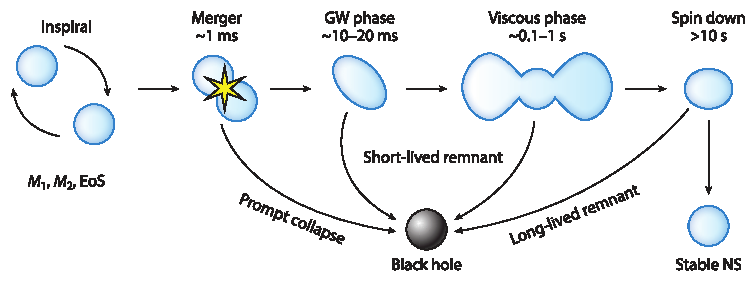
\includegraphics[width=0.70\textwidth]{Fig_3_Rad.pdf}
    \caption{
        Overview of the different phases in an \ac{NS} merger and the relative timescales. 
        The inspiral ends with the merger, when the two stars start to fuse together. 
        The early \pmerg{} evolution is entirely driven by hydrodynamics and by \ac{GW} emission. 
        If the remnant does not collapse within ${\sim}10-20\,$ms, \ac{GW} losses
        subside and other physical processes become more important: 
        Angular momentum redistribution (which is due to turbulent viscosity) 
        and neutrino losses operate over a timescale of a tenth of a second to a few
        seconds. This is also the characteristic timescale for the evolution of the remnant disk. 
        If the remnant does not collapse over a timescale of a few seconds, then it will 
        spin down because of \ac{MHD} effects over a possibly much longer timescale 
        of several seconds to a few hours. 
        (Adapted from \citet{Radice:2020ddv}).
    }
    \label{fig:intro:RadFig1}
\end{figure}


%% -----------------------------------
\section{Merger and \pmerg{}}\label{sec:intro:merg_pmerg} %ef in GRLESS
%% ------------------------------------

After \acp{NS} inspiral and merge, the dynamics of the system becomes significantly 
more complex, as temperature and density rise by orders of magnitude and new 
physical effects, \eg, magnetic fields and weak interaction, start to influence the evolution. 
The \pmerg{} phase is not well understood and mainly explored with miltiphsyics \ac{NR} 
simulations with various degrees of sophistication and resolution. 

The summary of the \ac{BNS} \pmerg{} evolution is shown in Fig.~\ref{fig:intro:RadFig1}. 
There are several trajectories that a system can take, depending when/if the formed remnant 
collapses to a \ac{BH}. The early \pmerg{} phase is charaterized by strong \ac{GW} 
emission and hydrodynamic effects. After it, several interlinked processes govern the 
evolution, \eg, \ac{MHD} stresses, that contribute to the angular momentum  redistribution, 
and neutrino emission, that alters the matter composition and cools i.
If \ac{BH} does not form, the \ac{MHD} torques and residual \ac{GW} emission spin down 
the remnant.

%% ------------------------------------------------
\subsection{Dynamics and Thermodynamics Conditions} \label{sec:intro:remnant}

Prior to the merger, \acp{NS} can be considered as being in the cold, neutrino-less, 
weak equilibrium with only marginal heating due to tidal deformation at the last orbits.
The dynamics at merger is dominated by the \acp{NS} orbital motion
as $\upsilon_{rad}\ll\upsilon_{orb}$, 
%\footnote{
%    The orbital speed can be written as $\upsilon_{orb}\eqsim\Omega r\eqsim\sqrt{GM/(R_A + R_B)}$
%    that for equal mass binary is $\upsilon_{orb}/c\eqsim\sqrt{C}\eqsim0.39(C/0.15)^{1/2}$.
%    The radial velocity is beven by the evolution of the orbital frequency, as 
%    $\omega_r \eqsim 2\Omega r \dot{\Omega}/(3\Omega^2)$. The $\dot{\Omega}$ can be 
%    estimated from the fact, that orbital frequency satisfies 
%    $\dot{\Omega}_{GW}\sim(3456/125)(G\mathcal{M}/c^3)^5\Omega_{GW}^{11}$ during the 
%    inspiral. Then, the radial velocity reads 
%    \begin{equation}
%    \upsilon_r/c\eqsim\frac{192\pi}{15}\frac{G^3 M^3}{c^5(R_A + R_B)^3}\frac{q}{(1+q)^2}
%    \end{equation}
%    that for equal mass gives $\upsilon_r/c \eqsim 0.0034 (C/0.15)^3$.
%}.
%Merger time, $t_{merg}$, estimated from the \ac{GW} frequency at \acp{NS} collisition 
%for comparable \ac{NS} masses is given by 
%\begin{equation}
%    t_{merg}\eqsim\frac{1}{2f_{GW}^{contact}}\eqsim1.50\text{ms}\Big(\frac{M}{2.8\,\Msun}\Big)^{1}
%\end{equation}
%where the frequency of \acp{GW} when \acp{NS} come into contact, \ie, when the distance 
%between them, $r = R_A + R_B$ can be evaluated from the Kepler law, given by 
%the quadrupolar gravitoelectric term, % Eq.~7
%$2GM\Omega \eqsim 2(M_B/(MC_B) + M_B/(MC_B))^{-3/2}$ \cite{29},
%as 
%\begin{equation}
%    f_{GW}^{contact} \eqsim 1.327 \Big(\frac{C}{0.15}\Big)^{3/2}\Big( \frac{M}{2.8\,\Msun} \Big) \text{ kHz}
%\end{equation}
that is $\upsilon_{orb}\eqsim\Omega r\eqsim\sqrt{GM/(R_A + R_B)}$.
This indicates that 
more compact binaries experience more rapid, more violent mergers.

%%%% Remnant
%When \acp{NS} collide, their deformed cores squeeze past each other, triggering \ac{KHI},
%in the first bounce. After several of these bounces, the cores fuse into a single object.
At collision, \ac{KHI} is triggered by the \acp{NS} cores plunging into the lower density matter of the companion, 
squeezing past each other and inducing the first wave of gravity-driven compression. 
The maximum values of temperatures and densities are reached than \citep{Perego:2019adq}. 
As nuclear and centrifugal forces start to dominate, the cores bounce back until gravity 
takes over again. %This is referred to as core \bnc{}. 
%
Notably, formed in the violent, fast collision, the remnant core, while being far from 
hydrodynamic equilibrium, does not exhibit shocks. This is due to high speed of sound 
of nuclear matter at supra-nuclear densities.
%($c_s\gtrsim0.2\, c$, at $\rho\gtrsim\rho_0$)
%
Shocks, however, do form at the remnant \ac{NS} surface, accelerating matter to mildly-relativistic 
velocities. %(\ref{Sec:intro:bns:ejecta}).
The fluid inside the cores remains cold 
%$T\lesssim10\,$MeV, $s\lesssim1\,k_B$/baryon 
throughout the merger, while at the interface between cores, the compression and shear 
dissipation raises the temperature to $T\sim70-110\,$MeV.
This is accompanied by the formation of the generic structure, described
by a pair of rotating hot regions, offset by $\sim\pi/2$ with 
respect to dense cold regions \citep{Kastaun:2016yaf}.
%
The subsequent evolution proceeds towards more axisymmetric, stable remnant, but can be 
interrupted by the \ac{BH} formation. 

%%%% Disk Foramtion
The matter outside the bouncing cores, lifted by tidal torques and squeezed out at the 
collisional interface, forms a disk (or a torus).
Due to various contributions with different properties, the disk is highly non-uniform.
The overall properties of the disk, such as mass, have complex dependency on 
binary parameters, that can be expressed, at a first approximation, via fitting 
formulae to \ac{NR} simulations \citep{Radice:2017lry,Radice:2018xqa,Radice:2018ozg}. 
The generic disk evolution around the remnant consists of quasi-adiabatic expansion
of its outer layers 
%with $T^3/\rho^3\sim\text{const}$ as the \ac{EOS} is dominated by non-relativisitc baryons
and cooling of the inner regions. 
%
However, as was mentioned above, the newly born \ac{NS} remnant is not hydrodynamically stable. 
Its dynamics is characterized by the pronounced $m=2$ bar- and $m=1$ one-armed-
deformations \citep[\eg][]{Radice:2016gym}, inducing spiral waves, propagating through the 
disk. 
%(see the Fig.~\ref{fig:ang_mom_flux} and related discussion in Ch.~\ref{ch:bns_sims}). % shocking and heating up the fluid. 
Additionally, the former leads to the strong \ac{GW} emission 
in ${\sim}10-20$~ms \pmerg{}. The backreaction from the energy and angular momentum 
loss dumps the $m=2$ mode efficiently and \ac{GW} emission subsides. 
%We refer to this evolutionary phase as \ac{GW}-dominated \pmerg{} phase.
%Notably, the $m=1$ mode, however, can persist due to mode coupling 
%\cite{Dietrich:2016phd}. 
That marks the end of the ``\ac{GW}-driven phase'' of the \pmerg{} evolution. 

%%%% Disk Settling down 
Weak processes and spiral density waves cool and shock periodically the 
fluid, bringing the disk to the configuration with an overall smooth 
temperature profile 
%from $\sim10\,$MeV at $\rho\eqsim10^{13}$\gcm to $\sim0.1\,$MeV at $\rho\eqsim10^4$\gcm
%with entropy $\in(3,10)$ $k_B$/baryon
and quasi-Keplerian orbit.
%
%%%% IF BH forms
If the remnant collapses to a \ac{BH}, the densest part of the disk is 
accreted on the dynamical timescale, reducing the total mass by half 
%and the disk maxiumum density to $\sim10^{12}\,$\gcm,
and disk shrinks \citep{Perego:2019adq}.

%%%% Magnetic fields
While \acp{MF} are not expected to affect the \ac{BNS} inspiral, their influence 
on the \pmerg{} evolution can be strong \citep{Duez:2006qe,Kiuchi:2017zzg}, as they get amplified 
to the values exceeding that of a magnetar 
%$10^{16}\,$Gauss, 
by a variety of processes, 
\eg, flux freezing and compression, \ac{KHI} at the collisional interface \citep{Kiuchi:2015sga},
\ac{MRI}, \citep{Duez:2006qe,Kiuchi:2017zzg} and \ac{MF} winding \citep{Duez:2006qe},

Whether the ordered, large-scale \acp{MF} can form in \pmerg{} environment 
via the dynamo process is presently unknown. They are important in producing 
polar collimated outflows, jets \citep{Bucciantini:2011kx,Ruiz:2016rai} and mildly relativistic 
outflows \citep{Metzger:2018qfl,Fernandez:2018kax}. Random magnetic fields are also 
relevant for the \pmerg{} evolution, as they generate stresses, enhancing angular momentum transport. 
Presently, these processes are not well understood, as seed \ac{MHD} instabilities operate at 
small scales (centimeters) and cannot be resolved in global \ac{MHD} \ac{BNS} merger 
simulations.
% with reslistic initial condiitons
To be able to resolve the instabilities (to increase their scale), the seed \acp{MF} are 
artificially enhanced to the magnetar-strength \citep{Kiuchi:2015sga,Kiuchi:2017zzg}.
%
%%%% Alpha-viscosity model
The effect of \acp{MF} on the angular momentum transport can be approximated via 
the $\alpha$-viscosity model \citep{Shakura:1972te}, calibrated 
with very high resolution \ac{MHD} simulations \citep{Radice:2017zta,Radice:2020ids}. 
%\red{More on it? For the theiry and GRLESS model?}
These effects are important 
in determining the remnant structure, lifetime and hence, the \pmerg{} \acp{GW} 
\citep{Radice:2017zta,Shibata:2017xht} 
%The timescale for the angular momentum redistribution in the remnant \cite{80} 
%\begin{equation}
%    t_{rem} \eqsim \alpha^{-1}R_{rem}^2\Omega_{rem}c_s^{-2}\eqsim 0.56\,s\Big(\frac{\alpha}{0.001}\Big)^{-1}\Big(\frac{R_{rem}}{15\,\text{km}}\Big)^2 \Big( \frac{\Omega_{rem}}{10^4\,\text{kHz}} \Big) \Big(\frac{c_s}{0.2\,c}\Big)^{-2}
%\end{equation}
%where $\Omega_{rem}$ and $c_s$ are the angular momentum and sound speed respectively.
as the loss of angular momentum brings the remnant closer to either stable, 
rigidly rotating configuration or collapse \citep{Hotokezaka:2013iia}. 
%
The \acp{MF} effects within the Keplerian disk facilitate accretion 
\citep{Fernandez:2015use,Fujibayashi:2017puw,Fernandez:2018kax,Miller:2019dpt}.
%on a timescale
%\begin{equation}
%    t_{disk} = \alpha^{-1}\Big(\frac{H}{R}\Big)^{-2}\Omega^{-1}_K \eqsim 0.78 \Big(\frac{\alpha}{0.02}\Big)^{-1}\Big(\frac{H/R}{1/3}\Big)^{-2}\Big(\frac{M_{rem}}{2.5\,\Msun}\Big)^{-1/2}\Big(\frac{R_{disk}}{100\,\text{km}}\Big)^{3/2}
%\end{equation}
%where $M_{rem}$ is the mass of the central remnant and $R_{disk}$ is the radial 
%scale of the disk.

%%%% Neutrinos
The prime cooling mechanism in the post-\ac{GW}-dominated phase is the emission of 
neutrinos, produced in hot, dense areas of the disk and remnant, and that are 
able to escape \citep{Eichler:1989ve,Rosswog:2003rv,Sekiguchi:2011zd}. 
%The typical neutrino mean free path is 
%\begin{equation}
%    \lambda_{\nu} = \Big(n_B\sigma_0(E_{\nu}/m_e c^2)^2\Big)^{-1}\simeq 24.6\,\text{m}\,(\rho/10^{14}\,\text{g}\,\text{cm}^{-3})^{-1}(E_{\nu}/10\,\text{MeV})^{-2},
%\end{equation}
%where $n_B$ is the density of baryons, and 
%\begin{equation}
%    \sigma_0 \simeq 4G_{F}^2 (m_e c^2)^2 / (\pi(\hbar c)^4)\simeq 1.76\times 10^{-44} \, \text{cm}^2
%\end{equation}
%is the typical neutrino cross section scale, and $E_{\nu}$ is the neutrino energy.
%Considering the charactersitic remnant temperature as  $T_{rem}\simeq20\,$MeV 
%energy of the thermal neutrinos then $E_{\nu}\simeq 3.15T_{rem}$ and optical depth 
%$\tau_{\nu}\simeq R_{rem}/\lambda_{\nu}=\mathcal{O}(10^{4})$.
The neutrinos are radiated on a diffusion timescale \citep{Perego:2014fma}.
%\begin{equation}
%    t_{diff} \simeq \frac{\tau_{\nu}R_{rem}}{c}\simeq 4.28\,s\Big( \frac{R_{rem}}{15\,\text{km}} \Big)^{-1}\Big(\frac{M_{rem}}{2.5\,\Msun}\Big)\Big(\frac{T_{rem}}{20\,\text{MeV}}\Big)^2.
%\end{equation}

%%%% neutrinos in the remnant and disk
Within the remnant, neutrinos are in a weak and thermal equilibrium with matter 
due to charged current reactions. There, the production of electron neutrinos, $\nu_e$,
is suppressed by degeneracy and as chemical potential $\mu_n-\mu_p+\mu_e<0$ at high temperatures, 
the electron anti-neutrinos, $\bar{\nu}_{e}$, dominate. The effect of these ``trapped'' 
neutrinos on the remnant evolution is not very strong \citep{Foucart:2015gaa,Perego:2019adq}.
%
Within the disk, however, the optical depth for neutrinos is ${\simeq}1$ so 
they can diffuse out on a timescale of milliseconds, lowering the disk 
temperature. The cooling rate is controlled by the degeneracy state of neutrinos 
%that is kept at mild values by the feedback negative effect, higher 
%values have on the cooling rate.
\citep{Beloborodov:2008nx}.

During the early \pmerg{}, the luminosity of the electron antineutrinos 
$L_{\bar{\nu}_e} \gtrsim L_{\nu_e}$, as the 
free neutrinos are abundant in the disk and the absorption opacity for $\nu_e$ 
exceeds that of $\bar{\nu}_e$.
Thus, alongside heating and decompression, the initially cold matter in weak 
equilibrium, undergoes \textit{leptonization} 
%The heavy neutrinos, $\nu_{\mu,\tau}$, are balanced by pair processes and 
%decouple from matter at higher densities and temperatures within the remnant
%namely $\rho\gtrsim10^{13}$\gcm and $T\gtrsim8\,$MeV 
\citep{Perego:2014fma,Endrizzi:2019trv},
%The, BNS simulations including
%neutrino transport predict the mean neutrino energies at infinity
%$E_{\nu_{e}}(\sim 10\,\text{MeV})\lesssim E_{\bar{\nu}_e}(\sim 15\,\text{MeV}) \lesssim E_{\nu_{\mu,\tau}}(\sim 20\,\text{MeV})$. Notably, binaries with higher mass 
%show higher neutrino energies \cite{14,86}.
\ie, $n+\nu_e\rightarrow p + e^-$. %\red{check that, from Wiki}
%
Neutrinos with different energies decouple from matter in different regions.
%due to the stron dependency of the cross section on the incoming neutrino energy.
Mildly energetic $\nu_{e}$ and $\bar{\nu}_e$ decouple at ${\sim}10^{11}\,$\gcm, found 
in the disk, while low energy neutrinos decouple at higher ${\sim}10^{13}\,$\gcm.
The geometric surface along which neutrinos decouple is usually called ``neutrino 
surface'' \citep{Perego:2014fma,Endrizzi:2019trv}.
%The dependency of the location and the geometry of this surface on the thermodynamics 
%conditions and neutrino energy facilitates the need to coherent treatment of the 
%strong and weak interactions over a broad span of densities and temepratures.
%The energy dependent (spectral) neutrino radiation trasport is required in 
%\ac{BNS} merger simulations

%%%% Neutrino oscillations
While it has been shown that neutrino flavor conversions may occur in the \ac{BNS} 
\pmerg{} environment, \eg, the matter-neutrino oscillations, induced by the 
the fact that $\bar{\nu}_e$ decouple at smaller radii then $\nu_{e}$ 
\citep[\eg][]{Zhu:2016mwa,Tian:2017xbr}, and fast-flavor conversions above the 
neutrino surface \citep{Wu:2017drk}, their impact on the properties of the ejected 
material remains largely unexplored.
%More works of neutrino quantum kinetics equations \cite{90,91}, that include 
%collisional integral and angular and energy distributions of neutrinos are required.

%%%% EOS 
One of the main unknowns with respect to \ac{BNS} mergers, is the high density part, 
$\rho \gtrsim \rho_0$ of the \ac{NS} \ac{EOS} \citep[\eg][]{Hebeler:2013nza,Oertel:2016bki}, that corresponds to the 
relevant thermodynamic degrees of freedom and nucleonic interactions. For instance, 
the emergence of the new species, \eg, hyperons, pions, muons, and nuclear 
resonances, would lower the matter degeneracy, and thus, soften the \ac{EOS} \citep[\eg][]{Fore:2019wib,Vidana:2010ip}.
Additionally, the emergence of the deconfined quark matter, due to \ac{QCD} phase transition,
would alter \ac{EOS} at very high temperatures and densities,
the effect that is not well understood \citep{Busza:2018rrf}.

%% ---------------------------------------
\subsection{Fate of the Remnant}

The end product of \ac{BNS} merger depends primarily on the binary parameters, (masses, 
\mr{}) and \ac{EOS}, and in particular, on the maximum supported mass of a non-rotating 
\ac{NS}, $M_{max}^{TOV}$ \citep{Shibata:2016}, as well as on the finite temperature and 
non-beta-equilibrium composition effects. 
%
The \ac{BH} formation directly at merger is usually referred to as \ac{PC}. 
The conditions for it  are not well understood. 
Simulations show that in equal mass binaries, \ac{PC} occurs if the total mass 
$M\gtrsim M_{thr} = k_{thr}M_{max}^{TOV}$, where $k_{thr}\in(1.3,\,1.7)$ that depends on 
\ac{EOS} \citep{Shibata:2005ss,Shibata:2006nm,Hotokezaka:2011dh,Bauswein:2013jpa}.
%(or $\kappa_2^T\lesssim43-73$, or $\tilde{\Lambda}\lesssim338-386$.
Simulations of unequal mass binaries show that the threshold is lower \citep{Bauswein:2017vtn}, 
and $k_{thr}\propto C_{1.6}$, with $C_{1.6}$ being the compactness of the $1.6\,\Msun$ 
\ac{NS} \citep{Hotokezaka:2011dh,Bauswein:2013jpa,Bauswein:2017vtn}. 
%As \ac{PC} cases are 
%not expected to ejecta large amount of material and be \ac{EM}-loud (in case of 
%comparable mass binary), the \GW{} is believed to be not a \ac{PC} case, 
%\cite{Margalit:2017dij,Bauswein:2017vtn}. 

A remnant that does not undergo \ac{PC} is a massive \ac{NS}, temporarily supported 
by fast rotation \citep{Baumgarte:1999cq,Rosswog:2001fh,Shibata:2005ss,Shibata:2006nm,
    Sekiguchi:2011zd,Hotokezaka:2013iia,Bernuzzi:2015opx}, whose lifetime depends 
intricately on the \ac{EOS}, finite temperature effects, and viscosity. A commonly 
adopted classification, based on the properties of equilibrium models (neglecting the 
dynamical, finite temperature, and magnetic effects), \ie, $M_{max}^{TOV}$ and
$M_{max}^{RNS}$\footnote{
    $M_{max}^{RNS}$ is the maximum mass of a rigidly rotating \ac{NS} (no differential 
    rotation) supported by zero-temperature (cold) \ac{EOS}. Also sometimes referred as 
    mass-shedding limit.
    % $M_{max}^{TOV}$ and $M_{max}^{RNS}$ are agnostic to thermal or magnetic eects 
    %which can impact the stability of the remnant in nontrivial ways (108, 72)
}
distinguishes between 
(i) \ac{HMNS} if $M>M_{max}^{RNS}$, 
(ii) \ac{SMNS} if $M_{max}^{TOV} \leq M_{max}^{RNS}$,
and (iii) stable \ac{MNS} if $M < M_{max}^{TOV}$ \citep[\eg][]{Baumgarte:1999cq}.
A \ac{HMNS} is supported by differential rotation that viscosity reduces with time 
and it is expected to collapse to a \ac{BH}. A \ac{SMNS} can avoid the collapse 
even after reaching rigidly rotating configuration. The lifetime of a \ac{HMNS} and 
a \ac{SMNS} depends on the efficiency of mass and angular momentum loss 
(to, \eg, \acp{GW} and massive winds) and finite temperature effects \citep{Radice:2018xqa}. 
%
Discussing the \ac{NR} simulations we shall distinguish between \textit{short-lived} remnants, 
that collapse to \ac{BH} during \ac{GW}-dominated phase, 
% taht correspods to ${\sim}10-20\,$ms after merger \cite{107,60}
and \textit{long-lived} remnants otherwise.

If a remnant can achieve rigid rotation, its evolution then is characterized by the emission 
of \acp{GW} (due to residual asphericity) and magnetic braking, reducing further its 
angular momentum, until either a \ac{BH} forms, or a stable non-rotating equilibrium is reached.
The observations of \acp{SGRB} with X-ray plateu 
\citep{Zhang:2000wx,Lasky:2015lej,Fan:2013cra}, which if indeed is a consequence of 
a magnetar activity\footnote{
    There are other possible explanations behind the X-ray plateu emission of \acp{SGRB} 
    \citep{Oganesyan:2019jij}
}, suggest that the remnant may survive from seconds to hours \citep{Fan:2013cra,Ravi:2014gxa}.
Most of the energy, ${\sim}10^{52}\,$erg, that a remnant needs to lose before collapsing, if indeed \ac{SGRB} is powered by the accretion onto a \ac{BH}, 
is believed to be carried away in form of \acp{GW}, as \ac{EM} observations of \GW{} suggest.
%This emission can be observed for the nearby event \cite{111}, priding direct information 
%on the remnant fate. However this emission was not observed for \GW{} \cite{67,68}

From \ac{EM} observations of the merger the fate of the remnant can be inferred, 
albeit in the model-dependent way. 
In case of \GW{}, the presence of such counterpart 
strongly disfavors \ac{PC}, as in that case the ejection of any significant amount 
of matter is not expected \citep{Margalit:2017dij,Bauswein:2017vtn,Radice:2017lry}, while leaving 
the question whether it was \ac{HMNS} or \ac{SMNS} open. \citet{Margalit:2017dij} suggested 
that the remnant was short-lived, on account of the non-detection of the expected ${\sim}10^{52}\,$erg, 
from the spin-down of the long-lived one. Assuming thus that \GW{} produced a \ac{HMNS}, 
allows to put a constraint $M_{max}^{TOV} \lesssim 2.2\,\Msun$ \citep{Margalit:2017dij}.
%
On the other hand, if the magnetar model of \acp{SGRB} is applied to \GW{} 
\citep{Ai:2018jtv,Li:2018hzy,Piro:2018bpl}, the remnant is required to be long-lived
(${\sim}$months) and exhibit weak dipol \acp{MF} \citep{Ai:2018jtv}, leading to a different 
constraint on the maximum mass of the non-rotating star, $M_{max}^{TOV} \gtrsim 2.2\,\Msun$. 
%and up to an order of magnitude lower ejecta mass ${\sim}10^{-3}\,\Msun$, that is attributed 
%to reducied amount of emergy from radioactive decay is required to explain the observed 
%UV/optical/infrared observations \cite{16}. 
%There have been indications of the X-ray flaring activity in \GRB{} \cite{117}, but 
%follow-up observations did not confirm it \cite{118}
 



%% --------------------------------------------------------------------------
%%               N U C L E O S Y N T H E S I S
%% --------------------------------------------------------------------------

\section{Ejecta, \nuc{}, electromagnetic counterparts}


For the discussion on \ac{EM} counterparts to mergers we refer to 
%For the most recent reviews on the topic we recommend the following reviews:
%Radice, for the discussing of the \pmerg{} dynamics and ejecta,
%Bernuzzis, for the \ac{GW} aspect of the mergers \cite{Bernuzzi:2020tgt}
%Shibata \& Hotokezaka for the discussing of the ejecta \cite{Shibata:2019wef}.
\citet{Kumar:2014upa,Fernandez:2015use,Metzger:2019zeh}.
%
%We conclude the chapter stating the aims and structure of this thesis.

%This chapter is organized as follows...
%First we discuss the observational context of the \ac{BNS} mergers, focusing on the 
%ejecta \nuc{} and \ac{EM} counterparts.
%Then we overview the current picture of \ac{BNS} mergers with emphasis on the 
%\pmerg{} dynamics and mass ejection mechanisms. 
%Finally, we state the goals of this thesis.


\subsection{$R$-process \nuc{}} \label{sec:intro:nucleo}

Nuclides with atomic number  $A\geq 56$ cannot be synthesized via nuclear burning 
due to their large Coulomb barriers and are produced via 
neutron capture processes \citep{Burbidge:1957}.
% Nucleosynthesis Cites
The maximum $A$ of a nuclide is limited by its binding energy, $Q_n$. 
At $Q_n \simeq1 \,$MeV photodisintegration starts breaking nuclides apart. 
The place in the parameter space of temperature and density where this occurs 
is called \textit{neutron drip line} \citep{Rolfs:1988}.
% Fast and Slow
Nuclides produced via neutron capture are generally unstable to $\beta$-decay,
and depending on whether the timescale for the decay is slower (faster) than 
the timescale of neutron capture, one distinguish rapid (slow) process called,
\rproc{} (\sproc{}).
%
The \sproc{} moves along the valey of stability, while \rproc{} moves along the 
neutron drip line.
%
When a nuclide reaches a closed neutron shell configuration, the cross-section 
for the subsequent neutron capture shrinks, and capture processes suspends until 
several $\beta$-decays take place. This results in the overproduction of nuclides 
that are located at the intersection between the neutron drip line and closed 
neutron shell for the \rproc{}. This manifests as ``peaks'' in the final abundance 
pattern at $A$ corresponding to these configurations.
Closed shell nuclides are located at $N=50,\: 82, \: 126$ and 
corresponding abundance peaks $A=80,\:130,\:194$ for \rproc{} 
(see \eg, \citet{Arnould:2007gh}).

%%%% R-proces cites
Conditions for the \rproc{} can be achieved in different astrophysical cites, \eg, 
certain types of \acp{SN} and \ac{BNS} mergers where very neutron rich (low 
electron fraction, $Y_e = 1/(1 + N_n/N_p)$, with $N_n$ and $N_p$ being the 
total proper number density of neutrons and protons respectively) 
conditions can be reached
\citep{Mathews:1990,Thielemann:2011,Lippuner:2015gwa,Siegel:2019mlp}. 
Regarding the \acp{SN}, winds driven by strong neutrino fluxes from the hot, deleptonized
core \citep{Qian:1996xt} were suggested as a promising cite \citep{Woosley:2002,Wanajo:2006mq}.
However, high $Y_e$ found in such winds do not allow for the full \rproc{} and only ``light'' heavy 
nuclide, up to $A\sim130$, can be synthesized 
\citep{Qian:1996xt,Thompson:2001ys,Fischer:2010,Roberts:2010,MartinezPinedo:2012rb,Wanajo:2013} 
%
A full \rproc{} can be achieved in so-called magnetorotationally driven \ac{CCSN},
(a rare type of \ac{CCSN} with a rapidly spinning strongly magnetized core), 
initiated by the \ac{MRI} and accompanied by a % magnetorotational processes \eg, 
formation of a 
collimated bipolar jet 
\citep{Wheeler:2000,Akiyama:2003,Burrows:2007yx,Mosta:2014jaa,Mosta:2015,Siegel:2019mlp}.
Conditions within such a jet were found to be suffient for full \rproc{} \nuc{} 
\citep{Winteler:2012,Nishimura:2015nca}.
%The rarity of this type of \acp{SN}, 
%however, might not allow for them to be the dominant source or \rproc{} material 
%\citep{Nishimura:2015nca} 

%Neutron-rich ejecta from \ac{BNS} and \ac{NSBH} mergers are regarded as one of 
%the main cites or \rproc{} \nuc{}.
%
%Mergers of two \acp{NS} or a \ac{NS} and a \ac{BH} are regarded as one of the main cites 
%of \rproc{} material.% (See Sec.~\ref{sec:intro:bns_merg}). 

%%%% Fission cycling
Under the very neutron-rich conditions, 
the nuclides beyond $A=300$ can be produced. Being unstable to fission, they 
decay into seed nuclides shortly after formation.
However, before they reach the valley of stability, neutron capture occurs again, and the cycle repeats.
This is so-called \textit{fission cycling}.
It is maintained as long as there are free neutrons, after which nuclides decay 
for the last time, forming a remarkably robust abundance pattern independent of the 
number of cycles (and thus on the exact conditions) 
(see figure 4 in \citet{Korobkin:2012uy}).

%%%% Cites
There is no consensus yet on what is the main source of \rproc{} material in the 
Universe. 
Observed \rproc{} abundances in \ac{MP} stars, formed early in the Galactic history, 
point towards a sources that was active in the early Universe, which is in tension with the long, 
$10^{6} - 10^{9}$ years, delay time required for compact object inspiral 
\citep{DeDonder:2004cx,Dominik:2012kk}. This estimate, however, depends strongly on the 
uncertain common envelop evolution phase of the massive binary (progenitors)
\citep[\eg][]{Dominik:2012kk}.
%
Observations of certain \acp{UFG} suggest that the stars there have been enrighed by rare, 
high-yield events (\eg, \ac{UFG} Reticulum II showed abundances similar to solar, 
while other \ac{UFG} galaxies show $2-3$ times lower abundances) \citep{Ji:2016}.
%
Earth crust and meteorites $^{244}$Pu studies also point towards rare, high-yield 
events \citep{Wallner:2015,Tsujimoto:2017}. This scenario has been confirmed with 
models of galactic mixing \citep{Hotokezaka:2015zea}.
%
It is however difficult to explain the observed uniform distribution of \rproc{} 
elements in the Galaxy with such events \citep{Argast:2003he}.
%
Population synthesis models have indicated that with a contribution from 
magnetorotationallydriven \acp{CCSN} the compact object mergers can account for the 
observed distribution \citep{Ishimaru:2015,Cescutti:2015,Wehmeyer:2015,VanDeVoort:2015}.



%% ----------------------------------








%% =====================================================================================
%%
%%              O R G A N I S A T I O N
%%
%% =====================================================================================

\section{Aims and organization of this thesis}

\ac{BNS} mergers and especially the \pmerg{} evolution hosts a number of interesting 
and yet poorly understood physics. Although there are many published \ac{NR} simulations of \ac{BNS} mergers, 
most of them are either very short, or neglect important physics, \eg, neutrino reabsorption, 
and effects of the \ac{MF}-induced turbulence. 
Moreover, the statistical analysis of up-to-date sample of thesis 
simulations is a pending task.
%
We intend to improve upon this situation by performing a large number of long-term ab-initio 
\ac{NR} \ac{BNS} simulations with neutrino reabsorption and viscosity, focusing on the 
\pmerg{} evolution of the remnant and astrophysical aspects, \ie, matter ejection, 
\rproc{} \nuc{} and \ac{EM} signals.
%
All simulations have chirp masses targeted to \GW{}, and with this work we aim to further 
constrain the \ac{NS} \ac{EOS} and the properties of the binary and shed light on 
some of the aforementioned discrepancies, namely the 
\begin{itemize}
    \item what is the long-term evolutionary trajectory of the \ac{HMNS} merger remnant
    \item whether the \ac{BNS} mergers are dominant cite of \rproc{}, 
    \item what is the additional ejecta component required to explain the blue \ac{kN} of \AT{}, 
    \item whether \ac{kN} afterglow from the ejecta of ab-initio \ac{NR} models is consistent with \GRB{} rebrightening.
\end{itemize}

The thesis is organized as follows.
In the Chapter \ref{ch:nr_methods} we provide a brief overview of the methods used to model  \ac{BNS} mergers, 
that are implemented in the code \wisky{}, used throughout this work.
In Chapter \ref{ch:bns_sims} we present the results of the simulations and discuss the \pmerg{} dynamics and ejecta.
In Chapter \ref{ch:nucleo} we compute the \rproc{} \nuc{} in the ejecta and compare the result with 
solar abundances.
In Chapter \ref{ch:kilonova} we compute the quasi-thermal \ac{EM} counterpart, \ac{kN}, and compare 
the synthetic light curves with the observations of \AT{}.
In Chapter \ref{ch:afterglow} we compute the non-thermal, \ac{kN} afterglow and compare the 
result the recently detected re-brightening of \GRB{}.
Finally, in Chapter \ref{ch:conclusion} we conclude our work and provide an outlook.